\appendix
% \npar\textbf{{\huge Appendix}}
\change{\npar In Appendix A, we first describe additional details about the participatory design process, as well as domain-specific artifacts collected from contextual inquiry. Next, in Appendix B, we articulate the space of problems amenable to VQSs and describe how the sensemaking processes introduced in Section~\ref{sec:sensemaking} into different parts of the problem space. Finally, in Appendix C, we provide supplementary information regarding our analysis methods and results.}
\section{Artifacts from Participatory Design\label{apdx:pdartifact}}
\change{Our collaboration with participants is illustrated in Figure~\ref{timeline}, where we began with an existing VQS (\zv, as illustrated in Figure~\ref{oldZV}) and incrementally incorporated features, such as dynamic class creation (Figure~\ref{dcc}), throughout the participatory design process.}
\begin{figure}[h!]
	\centering
	% \captionsetup{justification=centering,margin=2cm}
	\vspace{-10pt}
	% 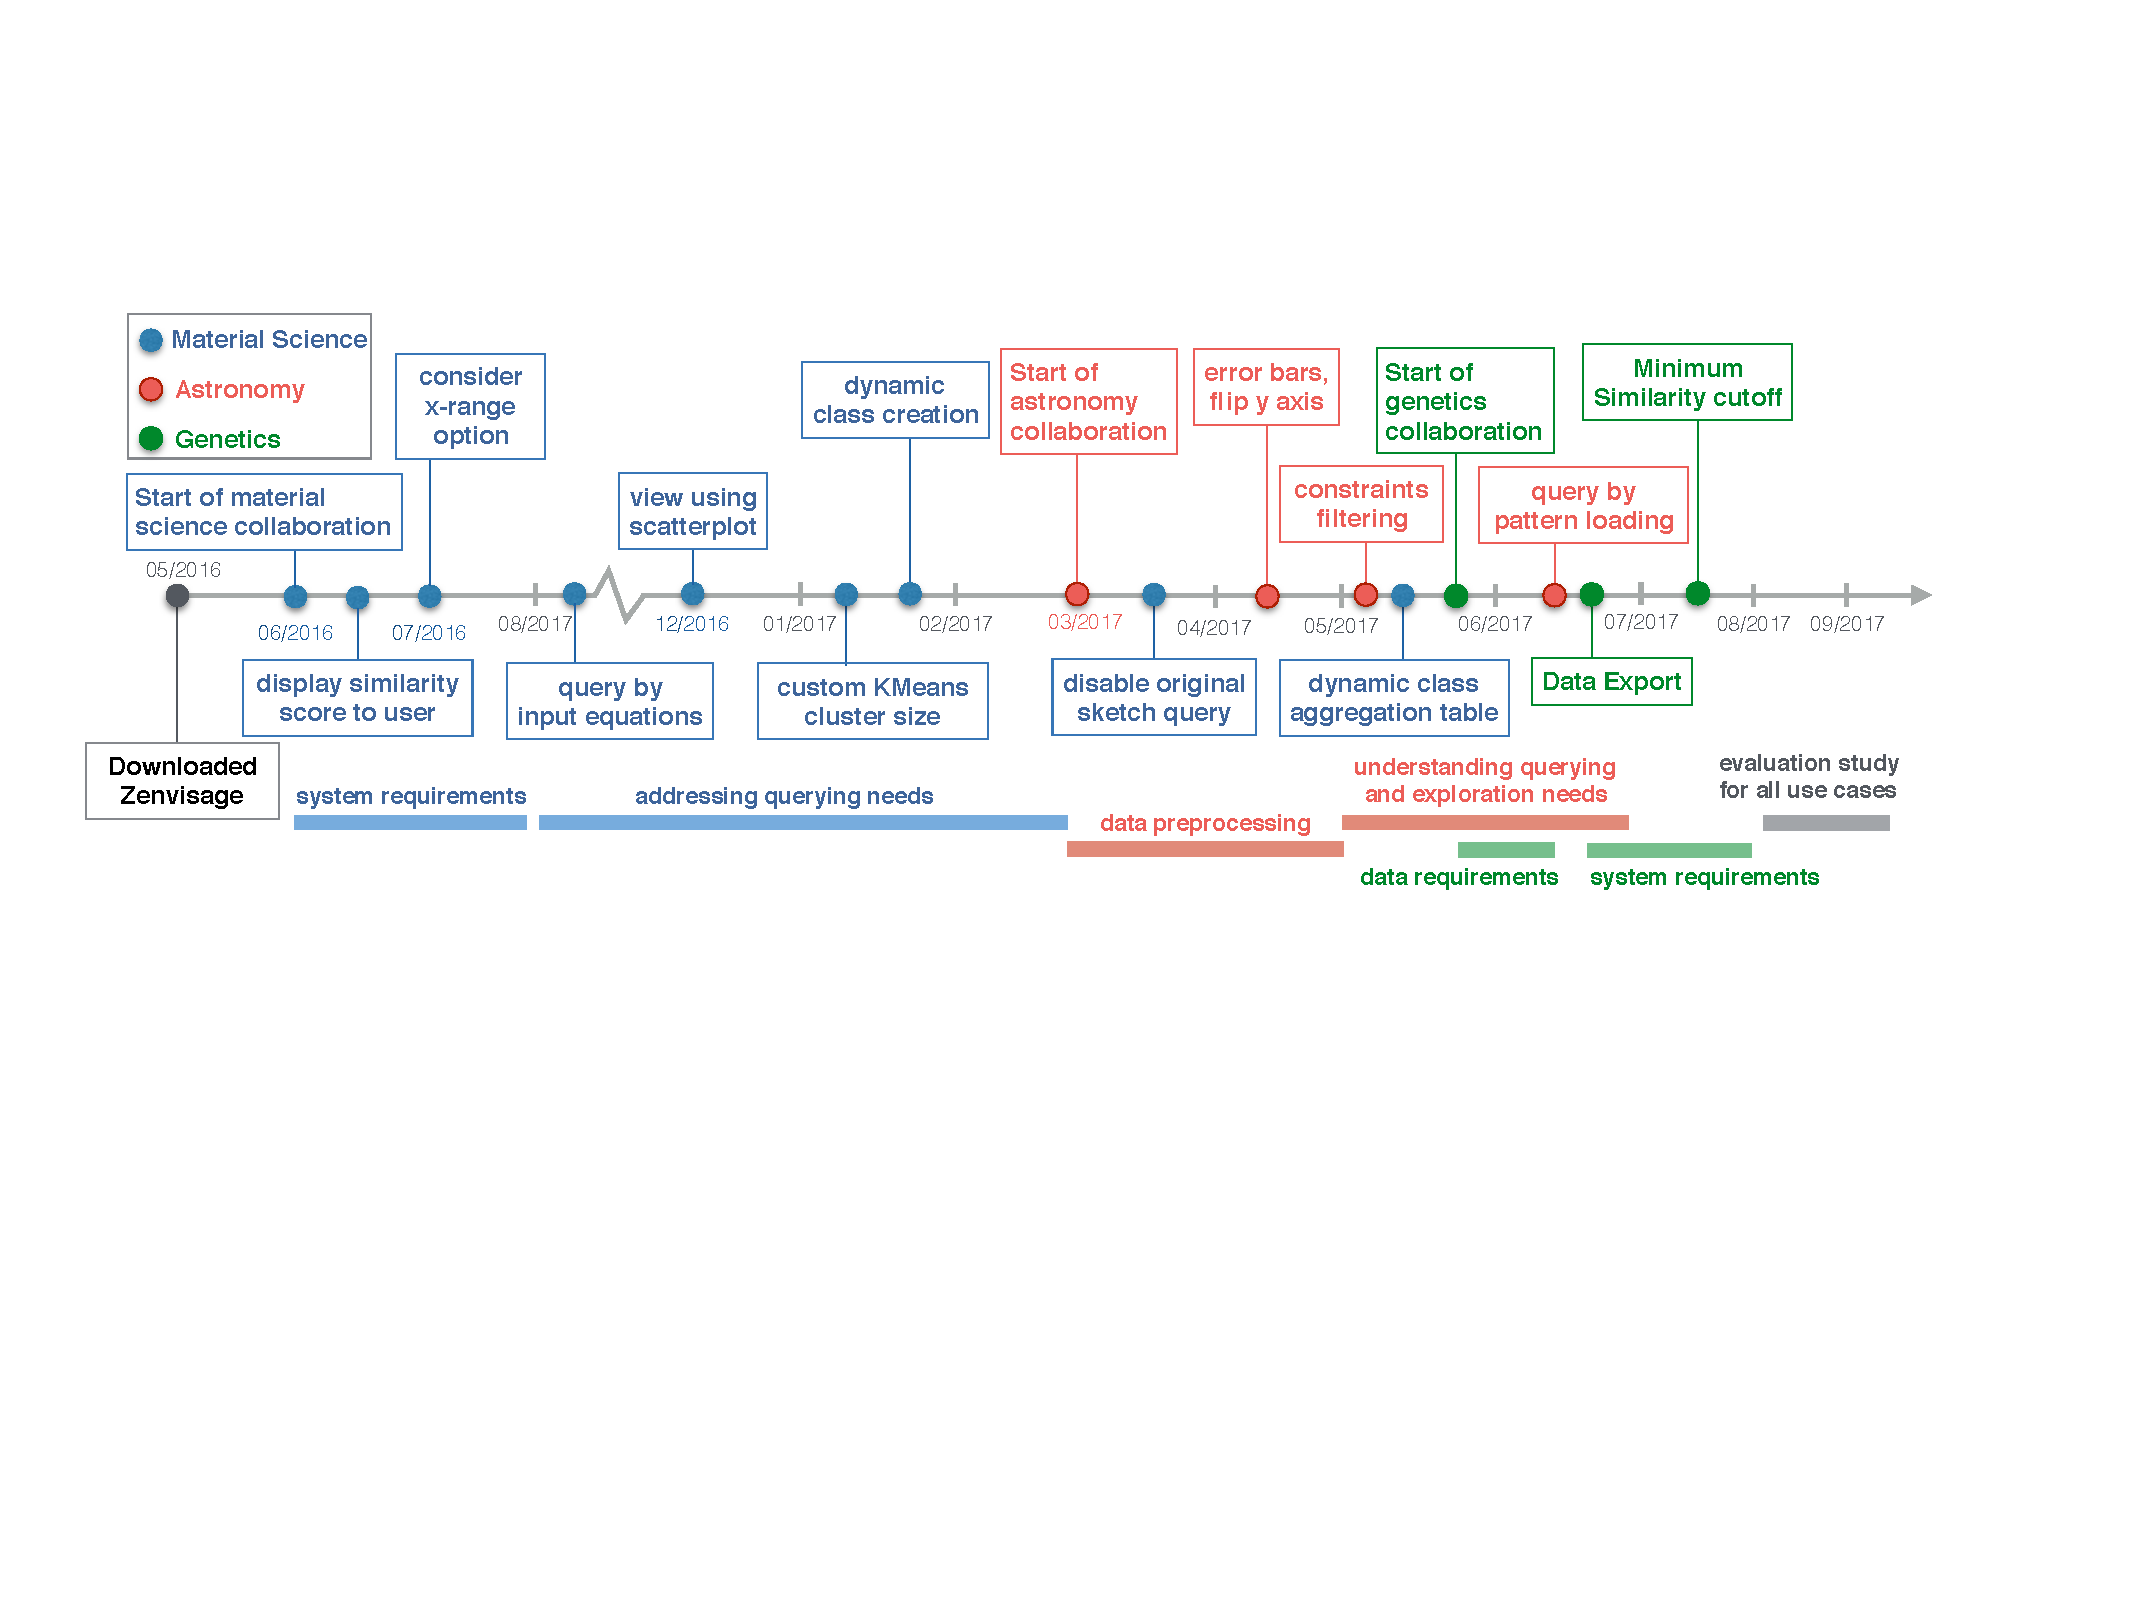
\includegraphics[width=6in]{figures/timeline.pdf}
  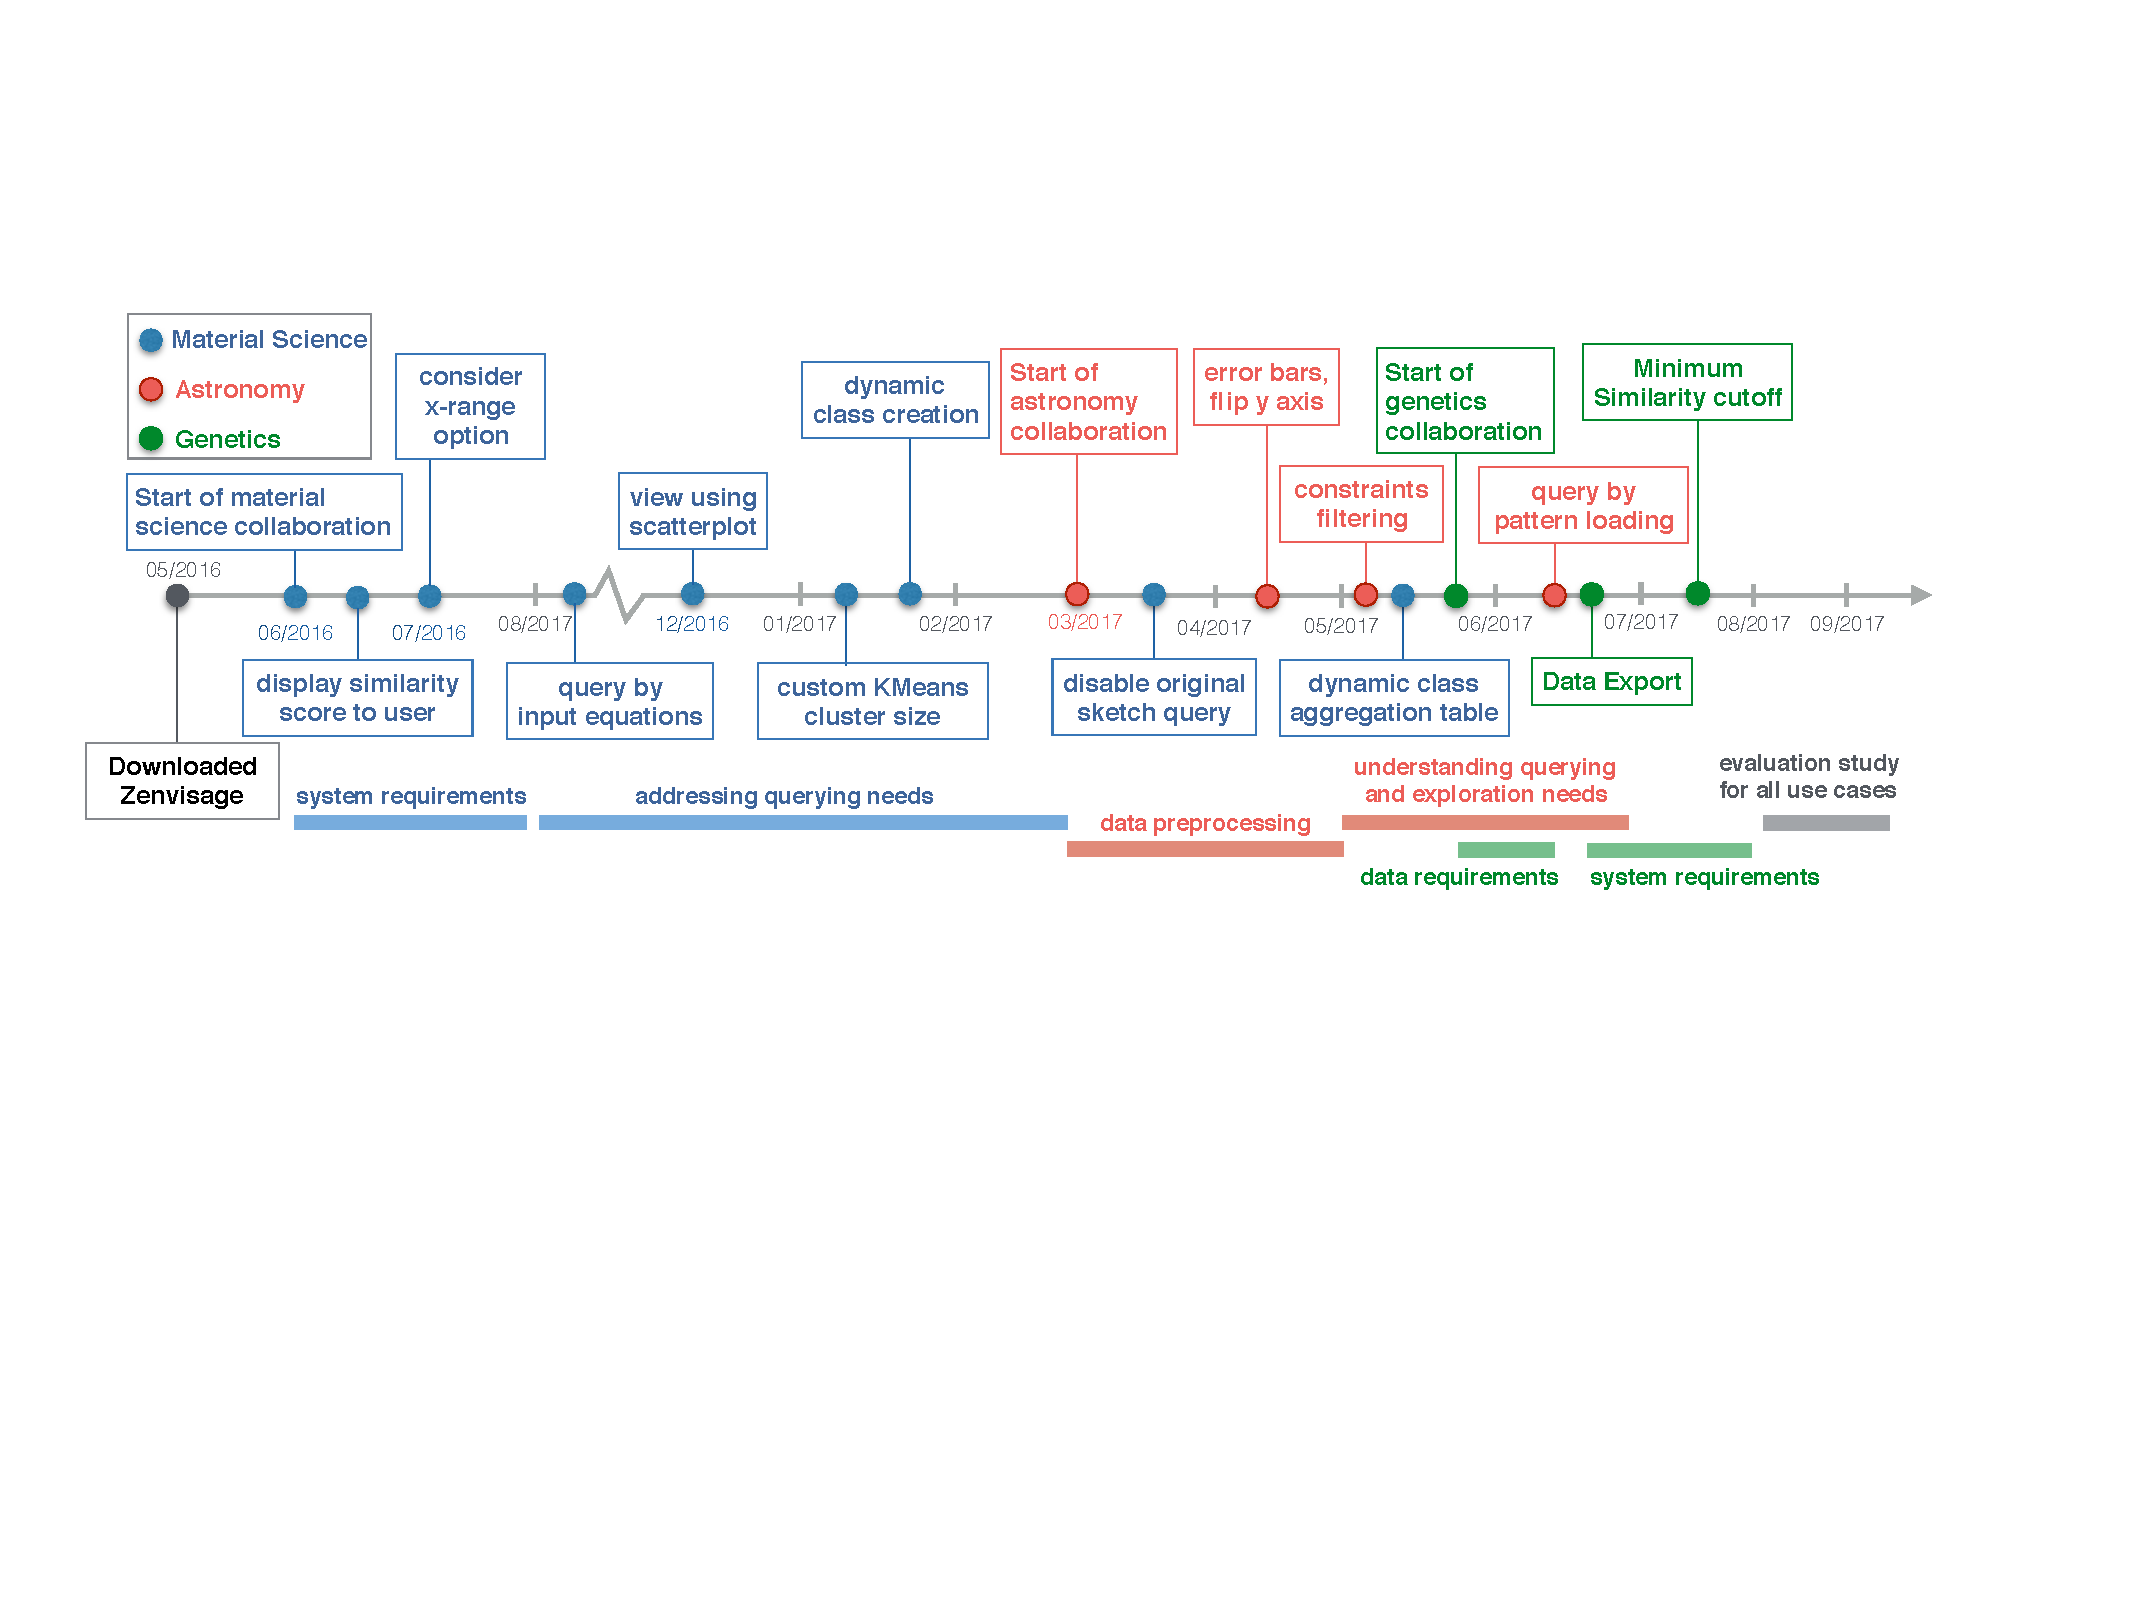
\includegraphics[width=\linewidth]{figures/timeline.pdf}
	\caption{Timeline for progress in participatory design studies.}
	\label{timeline}
	\vspace{-10pt}
\end{figure}
\begin{figure}[h!]
	\centering
	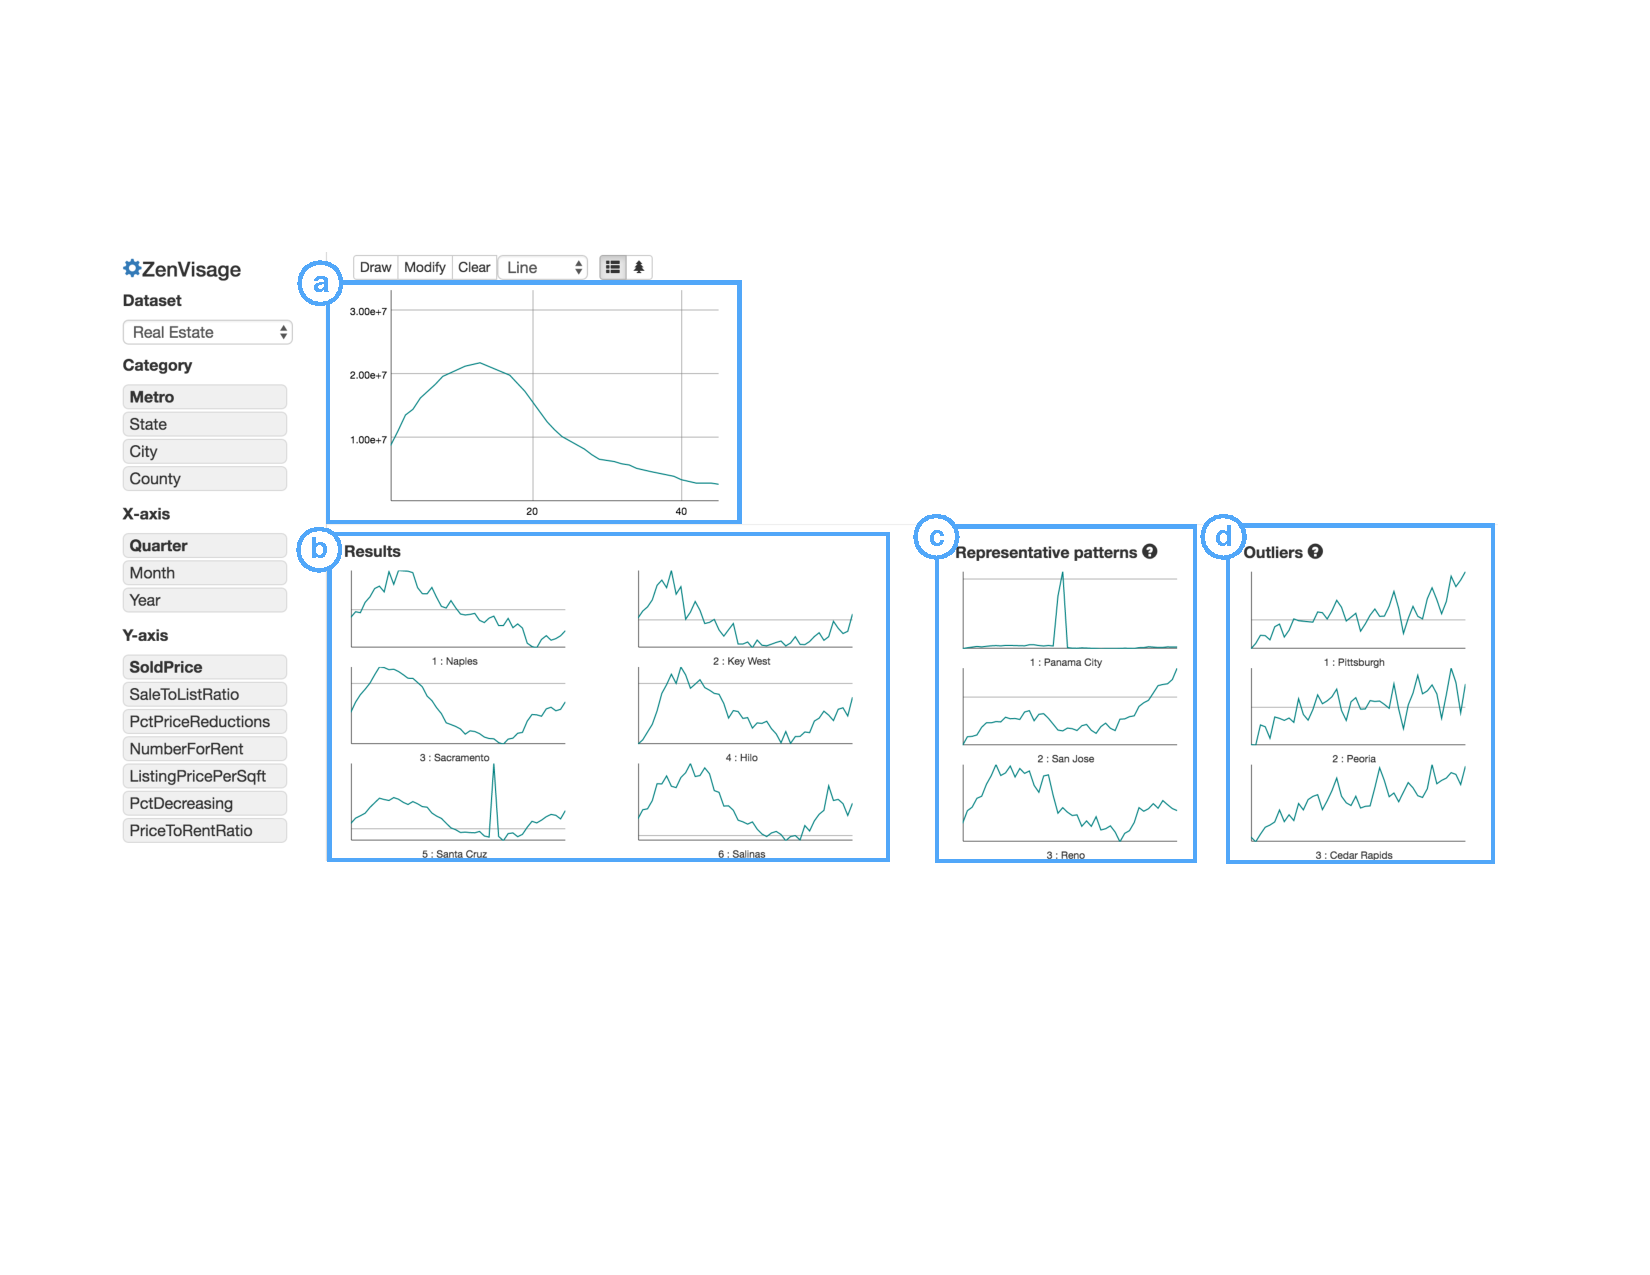
\includegraphics[width=0.9\linewidth]{figures/oldZV_nozql.pdf}
	\caption{The existing \zv prototype allowed users to sketch a pattern in (a), which would then return (b) results that had the closest Euclidean distance from the sketched pattern. The system also displays (c) representative patterns obtained through K-Means clustering and (d) outlier patterns to help the users gain an overview of the dataset.}
	\label{oldZV}
\end{figure}
\begin{figure}[h!]
  \centering
  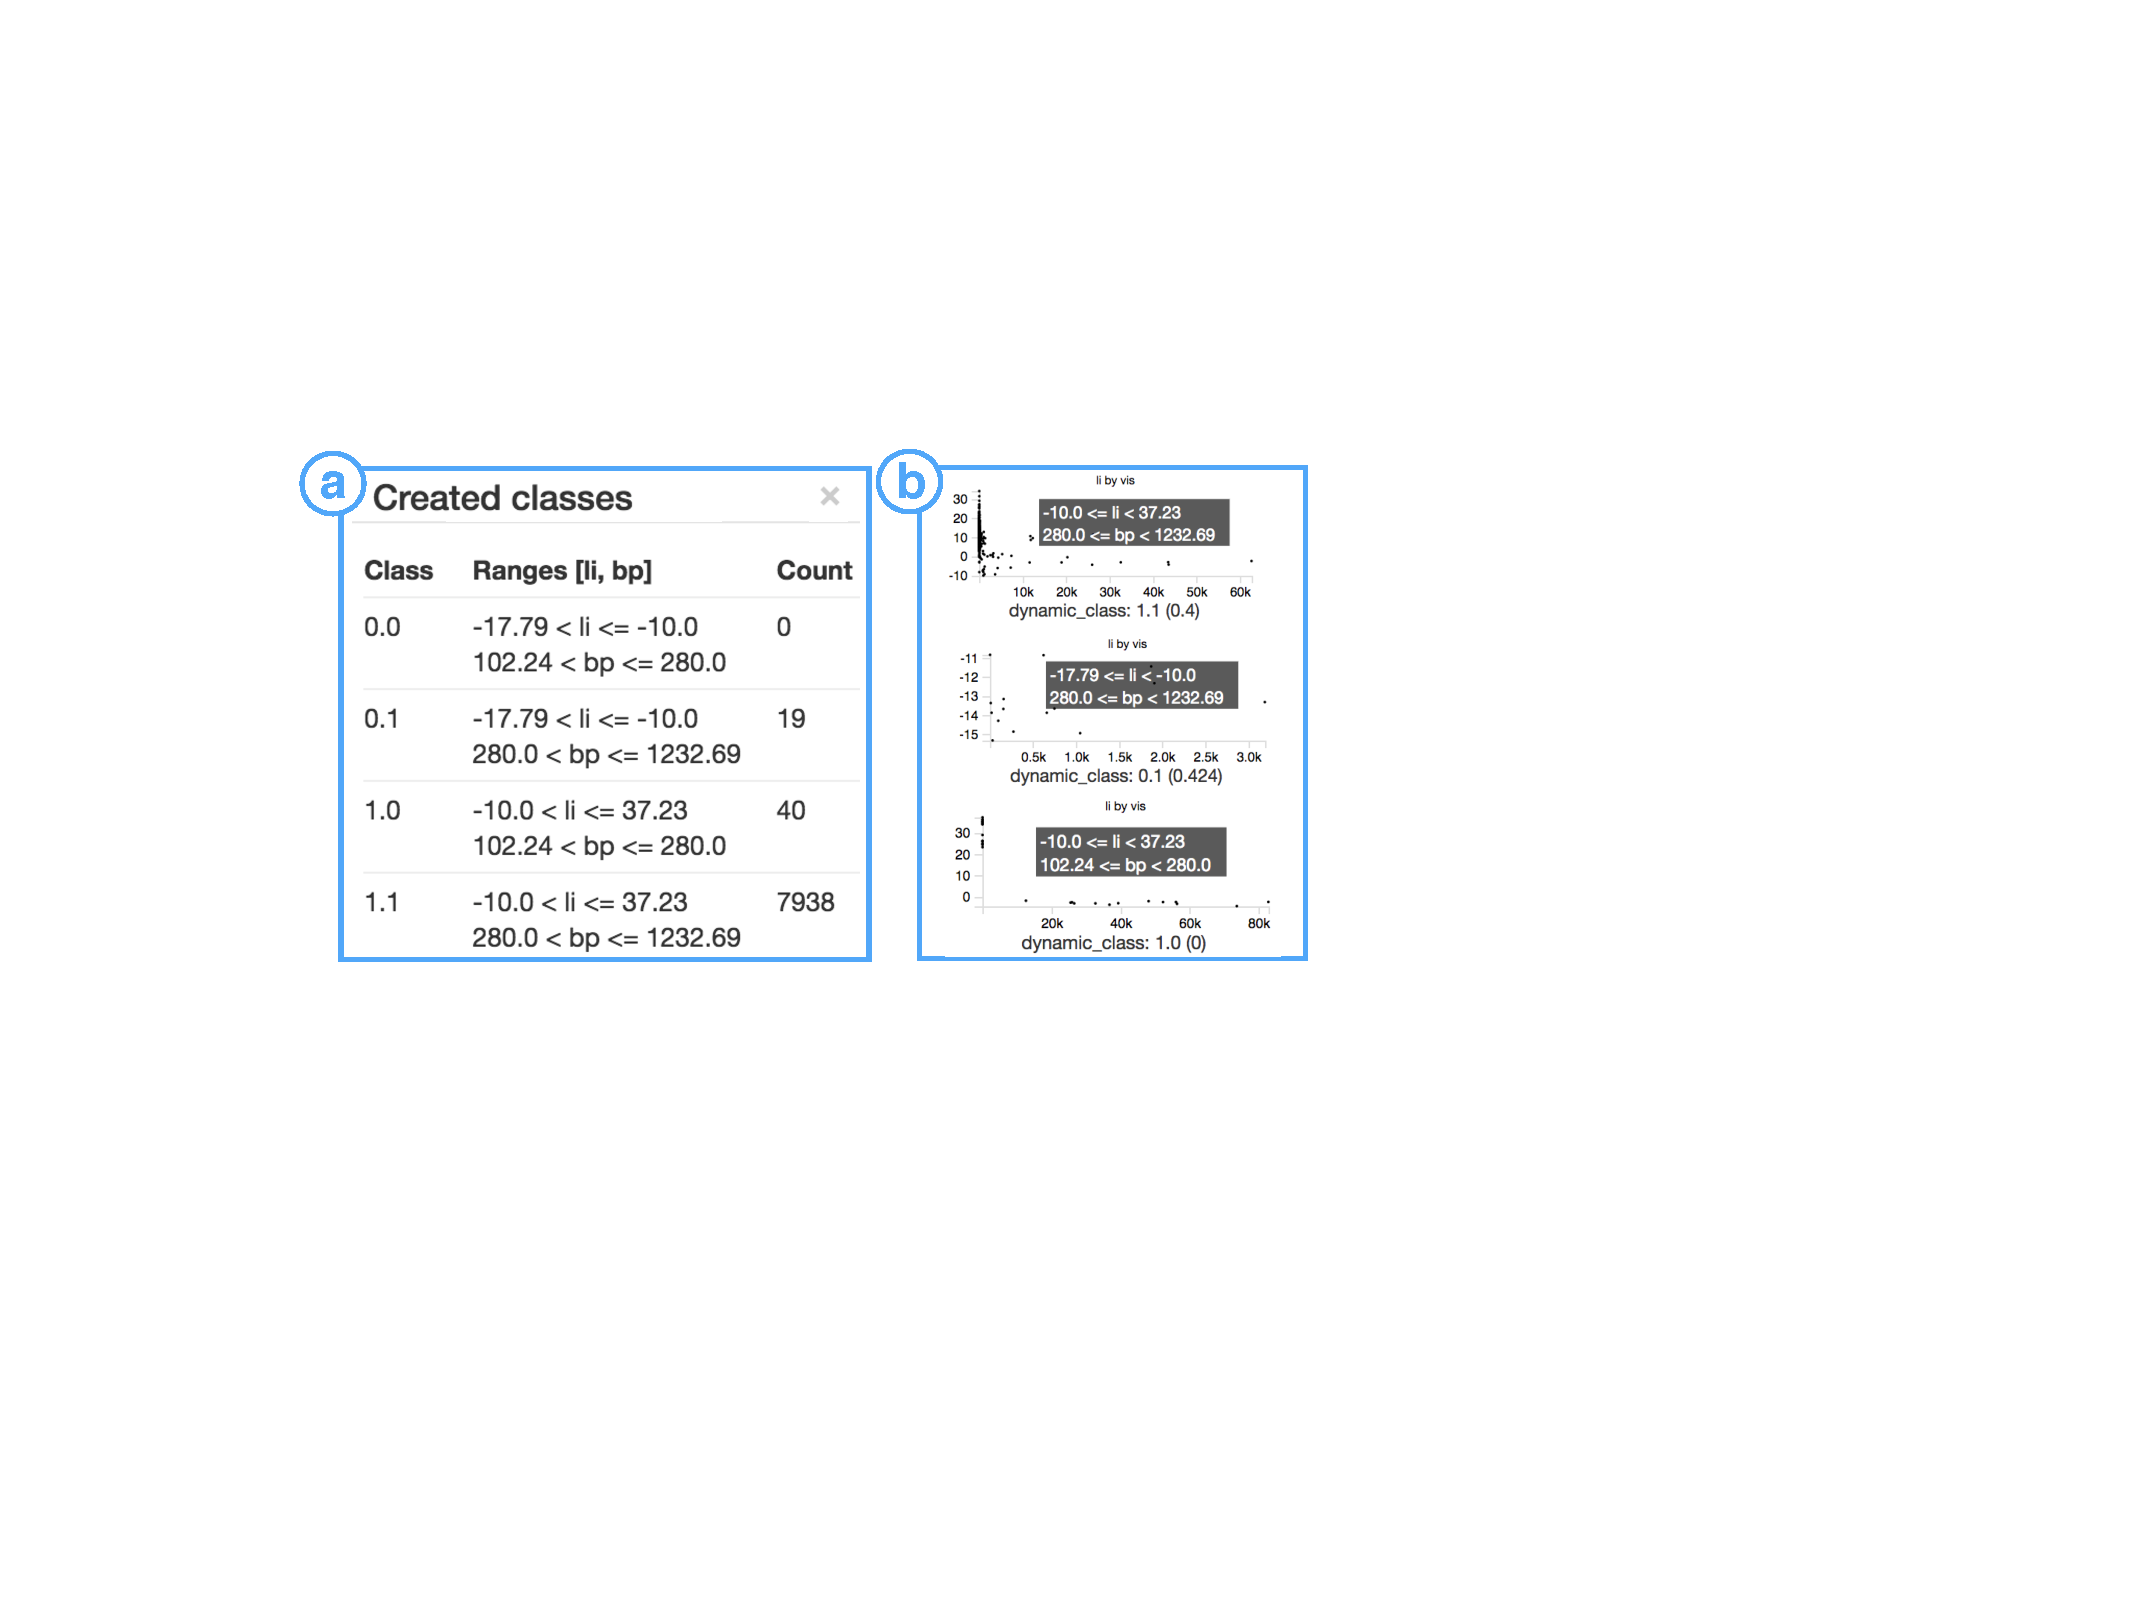
\includegraphics[width=0.9\linewidth]{figures/dcc.pdf}
  \vspace{-6pt}
  \caption{Example of dynamic classes. (a) Four different classes with different Lithium solvation energies (li) and boiling point (bp) attributes based on user-defined data ranges. (b) Users can hover over the visualizations for each dynamic class to see the corresponding attribute ranges for each class. The visualizations of dynamic classes are aggregate across all the visualizations that lie in that class based on the user-selected aggregation method.}
  \label{dcc}
  \vspace{-10pt}
\end{figure}
\newpage
\change{\npar During the contextual inquiry, participants demonstrated the use of external tools for conducting analysis in their existing workflow, as shown in Figure~\ref{workflow}, including:
  \begin{denselist}
    \item \href{http://descut.cosmology.illinois.edu}{Image Cutout Service (Astronomy)}
    \item \href{http://cs.cmu.edu/~jernst/stem/}{Short Time-series Expression Miner (Genetics)}
    \item \href{http://srdata.nist.gov/solubility/}{Solubility Database (Material Science)}
  \end{denselist}
}
\begin{figure}[h!]
  \centering
  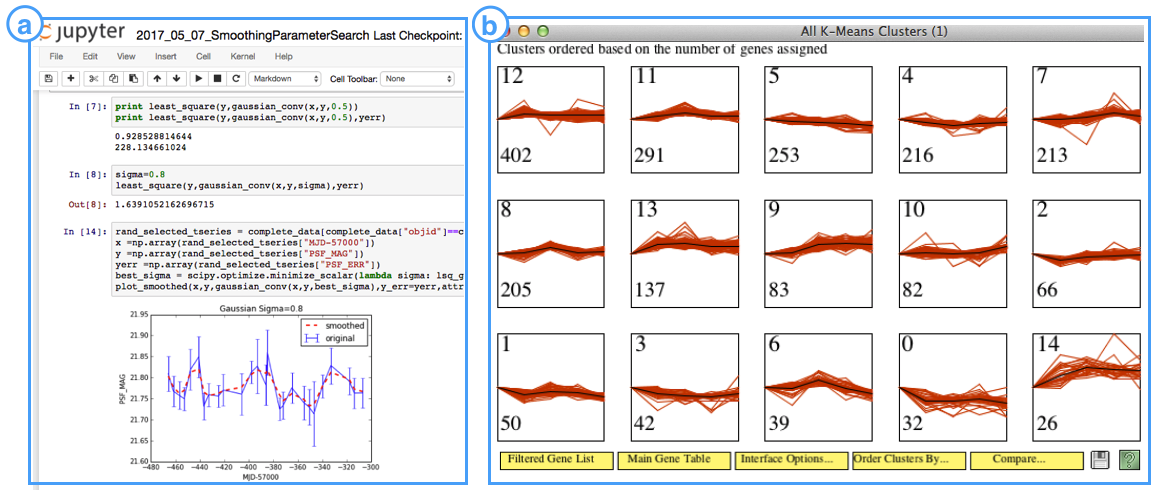
\includegraphics[width=0.9\linewidth]{figures/workflow.png}
  \caption{Screenshots from contextual inquiry: a) A1 examines a light curve manually using the Jupyter notebook environment, b) G2 uses a domain-specific software to examine clustering outputs.}
  \label{workflow}
\end{figure}
\vspace{-5pt}
\npar Based on our meeting logs with participants, we found that reasons for not carrying a feature from the design to implementation stage included:
\begin{denselist} %he amount of nice-to-have features that one could envision for the tool is endless.
\item Nice-to-haves: One of the most common reasons for unincorporated features comes from participant's requests for nice-to-have features. To this end, we use two criteria to heuristically judge whether to implement a particular feature:
\begin{enumerate}[leftmargin=*]
\item \textit{Necessity:} Without this feature, can participants still work with this dataset using the tool and meet their information needs?
\item \textit{Generality:} Will this feature benefit only this specific use case or be potentially useful for other domains as well?
\end{enumerate}
\item ``One-shot'' operations: We decided not to include features that only needed to be performed once and remain fixed thereafter in the analysis workflow. For example, certain preprocessing operations such as filtering null values only needed to be performed once with an external tool.
\item Substantial research or engineering effort: Some proposed features did not make sense in the context of VQS or required a completely different set of research questions. For example, the question of how to properly compute similarity between time series with non-uniform number of datapoints arose in the astronomy and genetics use case, but requires the development of a novel distance metric and algorithm that is out of the scope of our design study objective. %. For example, M3 proposed functional fitting to obtain fitting coefficients. Other features
\item Underdeveloped ideas: Other feature requirements came from casual specification that were underspecified. For example, A1 wanted to look for objects that have deficiency in one band and high emission in another band, but the scientific definition of ``deficiency'' in terms of brightness levels was ambiguous.
\end{denselist}
\change{\npar Figure~\ref{science_task} illustrates how each of the subtasks in participant's workflow can be addressed by a sensemaking process.}
\begin{table}[h!]
	\centering
	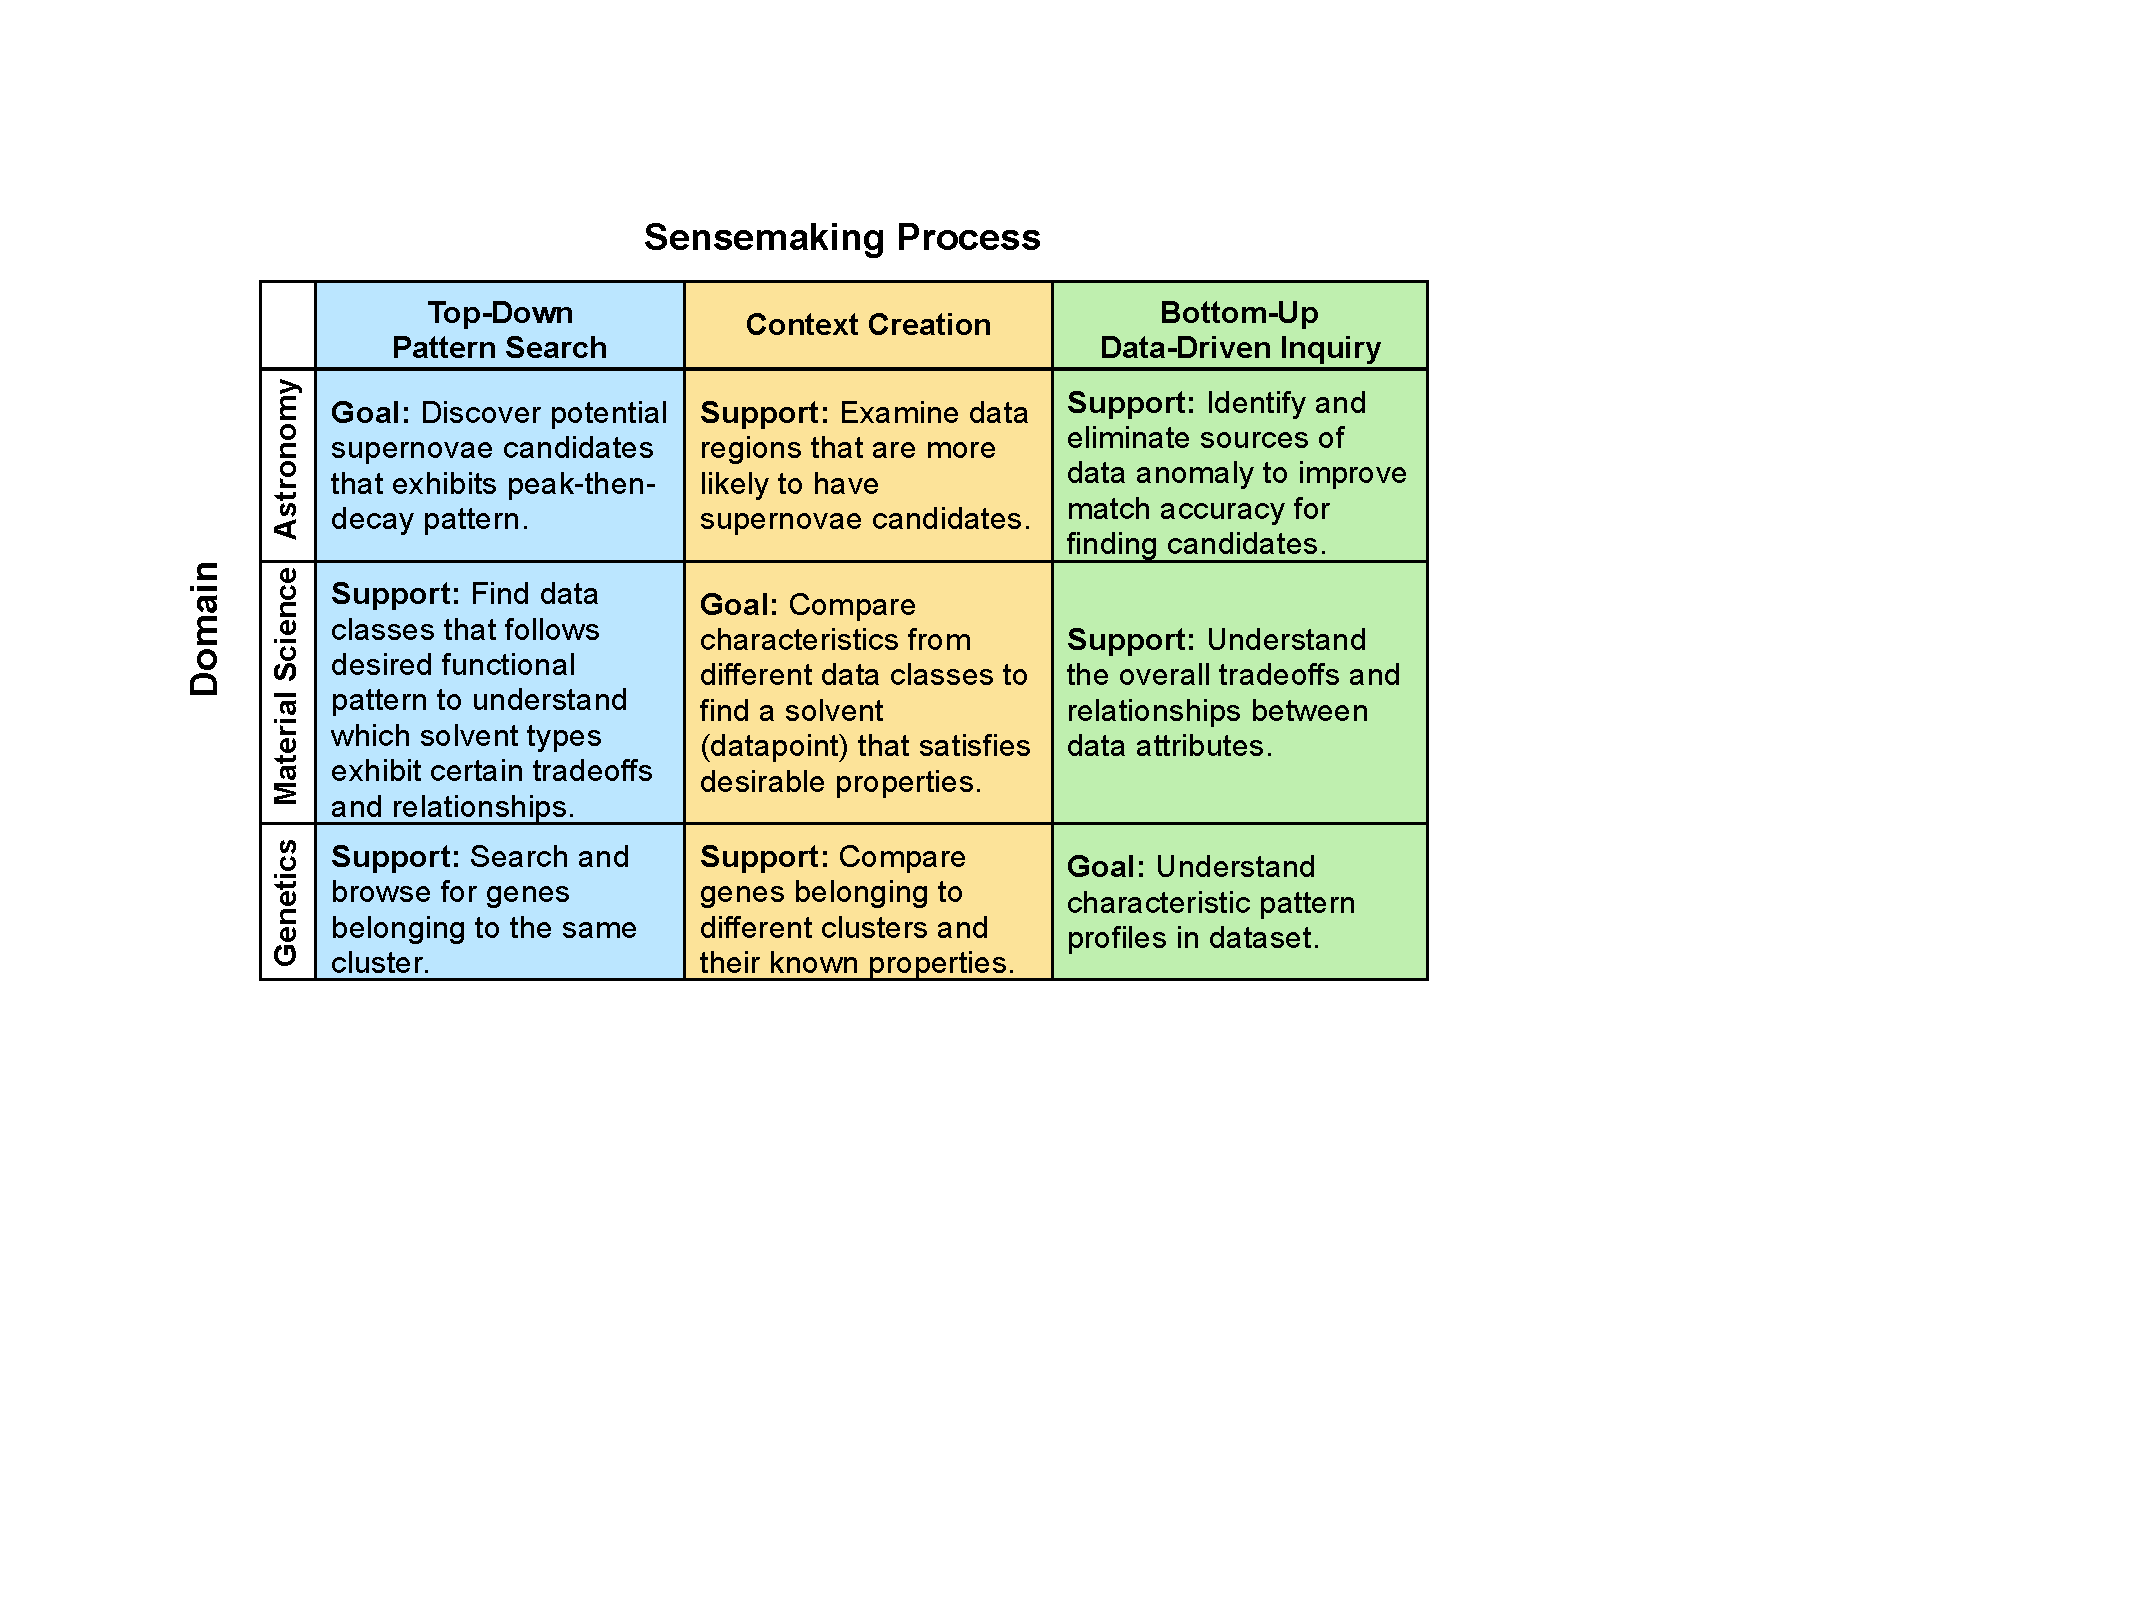
\includegraphics[width=\linewidth]{figures/science_task.pdf}
	\vspace{-6pt}\caption{Each VQS sensemaking process maps to scientific tasks and goals from each use case, from pattern search to comparing visualization collections to gaining overall data understanding. We find that our scientific participants typically have one focussed goal expressible through a single sensemaking process, but since their desired insights may not always be achievable with a single operation, they make use of the two other sensemaking processes to support them in accomplishing their main goal.}
	\label{science_task}
	\vspace{-10pt}
\end{table}

\section{Characterizing the Problem Space for VQSs}
We now characterize how each sensemaking process fits into different problem areas that VQSs are aimed to solve. Visual querying often consists of searching for a desired pattern instance (Z) across a visualization collection specified by some given attributes (X,Y). Correspondingly, we introduce two axes depicting the amount of information known about the visualized attribute and pattern instance.
\par Along the \textbf{pattern instance} axis, the visualization that contains the desired pattern may already be \texttt{known} to the analyst, exist as a pattern \texttt{in-the-head} of the analyst, or \change{be} completely \texttt{unknown} to the analyst. In the \texttt{known} pattern instance region (Figure~\ref{2dmodel} grey), visualization-at-a-time systems such as Tableau, where analyst manually create and examine each visualization one at a time, is more well-suited than VQSs, since analysts can directly work with the selected instance without the need for visual querying. Inspired by Pirolli and Card's information foraging framework~\cite{Pirolli}, which distinguishes between information processing tasks that are \textit{top-down} (from theory to data) and \textit{bottom-up} (from data to theory), we define \textit{top-down pattern search} as \change{the process where analysts query a fixed collection of visualizations based on their in-the-head pattern (Figure~\ref{2dmodel} blue)}. On the other hand, \change{\textit{bottom-up data-driven inquiries} (Figure~\ref{2dmodel} green) are driven by recommendations or queries that originate from the data (or equivalently, the visualization), since the pattern of interest is unknown and external to the user.} As we will discuss later, this process is crucial but underexplored in past work on VQSs.
%analysts often do not start with a known pattern instance. T
\par The second axis, \textbf{visualized attributes},
depicts how much the analyst
knows about which X and Y axes
they are interested in visualizing.
In both the astronomy and genetics use cases,
as well as past work in this space, \change{the attribute to be visualized is \texttt{known}, as data was in the form of a time series.} In the case of our material science participants, they wanted to explore relationships between different
X and Y variables. In this realm of \texttt{unknown} attributes, context creation (Figure~\ref{2dmodel} yellow) is
essential for allowing users to pivot across different visualization collections.
\begin{figure}[h!]
  \centering
  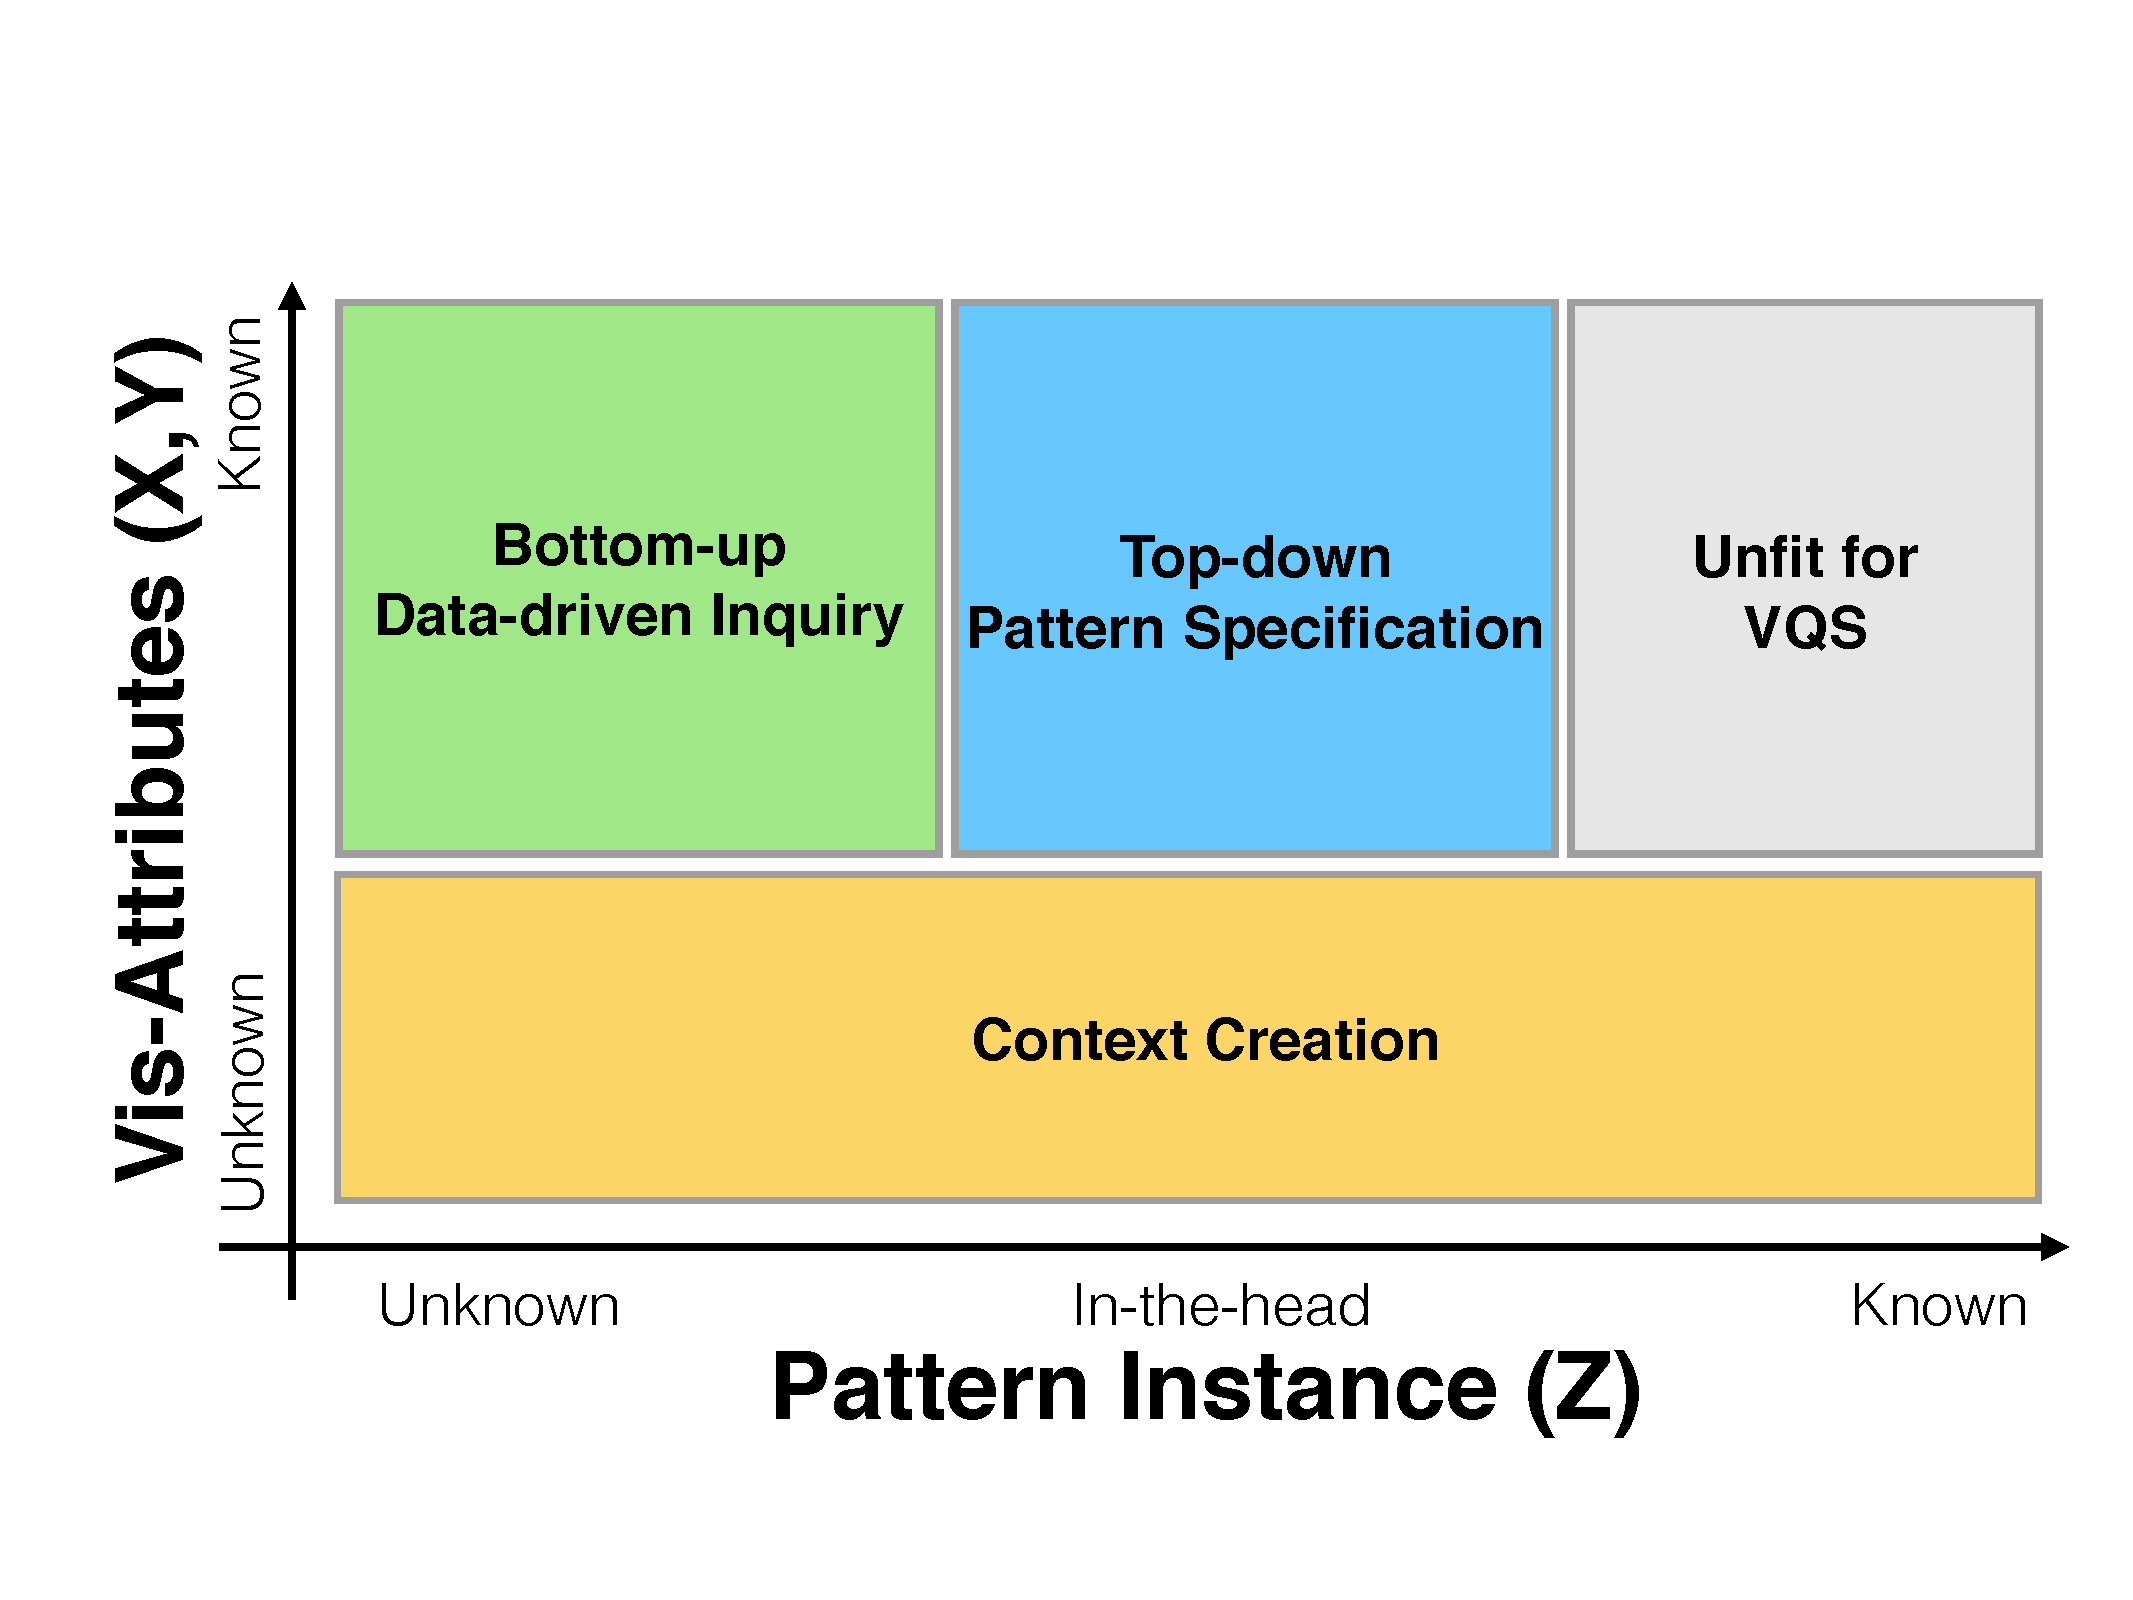
\includegraphics[width=0.9\linewidth]{figures/2dmodel.pdf}
  \caption{The problem space for VQSs is characterized by how much the analyst knows about the visualized attributes and the pattern instance. Colored areas highlight the three sensemaking processes in VQSs for addressing these characteristic problems. While prior work has focused solely on use cases in the blue region, we envision opportunities for VQSs beyond this to a larger space of use cases covered by the yellow and green regions.}
  \label{2dmodel}
  \vspace{-10pt}
\end{figure}

\section{Evaluation Study Analysis Details\label{apdx:studydetails}}
We analyzed the transcriptions of the evaluation study recordings through open-coding and
categorized every event in the user study using the following coding labels:
\begin{denselist}
    \item Insight (Science) \textbf{[IS]}: Insight that connected back to the science (e.g. ``This cluster resembles a repressed gene.'')
    \item Insight (Data) \textbf{[ID]}: Data-related insights (e.g. ``A bug in my data cleaning code generated this peak artifact.'')
    \item Provoke (Science) \textbf{[PS]}: Interactions or observations that provoked a scientific hypothesis to be generated.
    \item Provoke (Data) \textbf{[PD]}: Interactions or observations that provoked further data actions to continue the investigation.
    \item Confusion \textbf{[C]}: Participants were confused during this part of the analysis.
    \item Want \textbf{[W]}: Additional features that participant wants, which is not currently available on the system.
    \item External Tool \textbf{[E]}: The use of external tools outside of \zvpp to complement the analysis process.
    \item Feature Usage \textbf{[F]}: One of the features in \zvpp was used.
    \item Session Break \textbf{[BR]}: Transition to a new line of inquiry.
\end{denselist}

\begin{table}[h!]
  \begin{tabular}{lrrrrrrrrr}
  \hline
   Domain           &   IS &   ID &   PS &   PD &   C &   W &   E &   BR &   F \\
  \hline
   astro            &    4 &   12 &   13 &   57 &   2 &  18 &  20 &   22 &  67 \\
   genetics         &    8 &   12 &    7 &   35 &   4 &  13 &   1 &   21 &  52 \\
   mat sci          &   14 &    8 &    7 &   44 &   8 &  11 &   3 &   12 &  48 \\
  \hline
  \end{tabular}
  \caption{Count summary of thematic event code across all participants of the same subject area.}
\end{table}
\npar In addition, based on the usage of each feature during the user study, we categorized the features into one of the three usage types:
\begin{denselist}
    \item Practical \textbf{[P]}: Features used in a sensible and meaningful way.
    \item Envisioned usage \textbf{[E]}: Features which could be used practically if the envisioned data was available or if they conducted downstream analysis, but was not performed due to the limited time during the user study.
    \item Not useful \textbf{[N]}: Features that are not useful or do not make sense for the participant's research question and dataset.
\end{denselist}
The feature usage labels for each user is summarized in Figure~\ref{feature_heatmap}. A feature is regarded as \emph{useful} if it has a \textbf{P} or \textbf{E} code label. Using the matrix from Figure~\ref{feature_heatmap}, we compute the percentage of useful features for each sensemaking process as: $\frac{\textrm{\# of useful features in process}}{\textrm{total \# of features in process} \times \textrm{total \# of users}}$.
\vspace{-10pt}
\begin{figure}[h!]
    \centering
    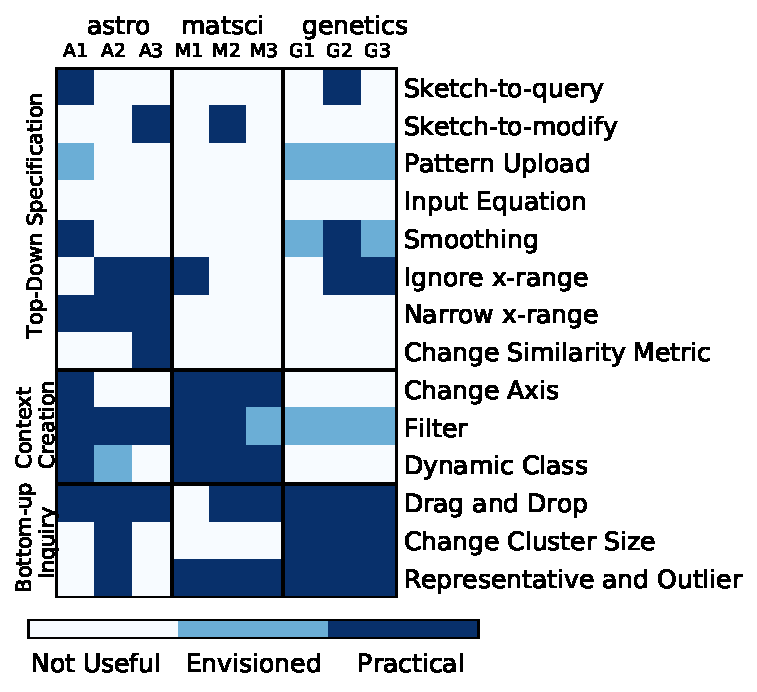
\includegraphics[width=0.7\columnwidth]{figures/PENcoding.pdf}
    \vspace{-6pt}\caption{Heatmap of features categorized as practical usage (P), envisioned usage (E), and not useful (N). Columns are arranged in the order of subject areas and the features are arranged in the order of the three foraging acts. Participants preferred to query using bottom-up methods such as drag-and-drop over top-down approaches such as sketching or input equations. Participants found that context creation via filter constraints and dynamic class creation were powerful ways to compare between subgroups or filtered subsets.}
    \label{feature_heatmap}
    \vspace{-5pt}
\end{figure}
